Funkční požadavek \textbf{\ref{F1}} byl na základě provedené rešerše \ref{zvyraznovani-syntaxe} realizován vytvořením
TextMate gramatiky. Tato gramatika je tvořena \textit{grammar} souborem ve složce \mintinline{text}{grammars}. Dynamické
tvorby gramatiky za pomoci API prozatím nebylo využito, její použití zůstává možným vylepšením do budoucna. Zvýrazňování
syntaxe WooWoo zdroje studijního textu k BI-PKM lze vidět na obrázku \ref{zvyraznovani-syntaxe-pkm}.

\begin{figure}\centering
    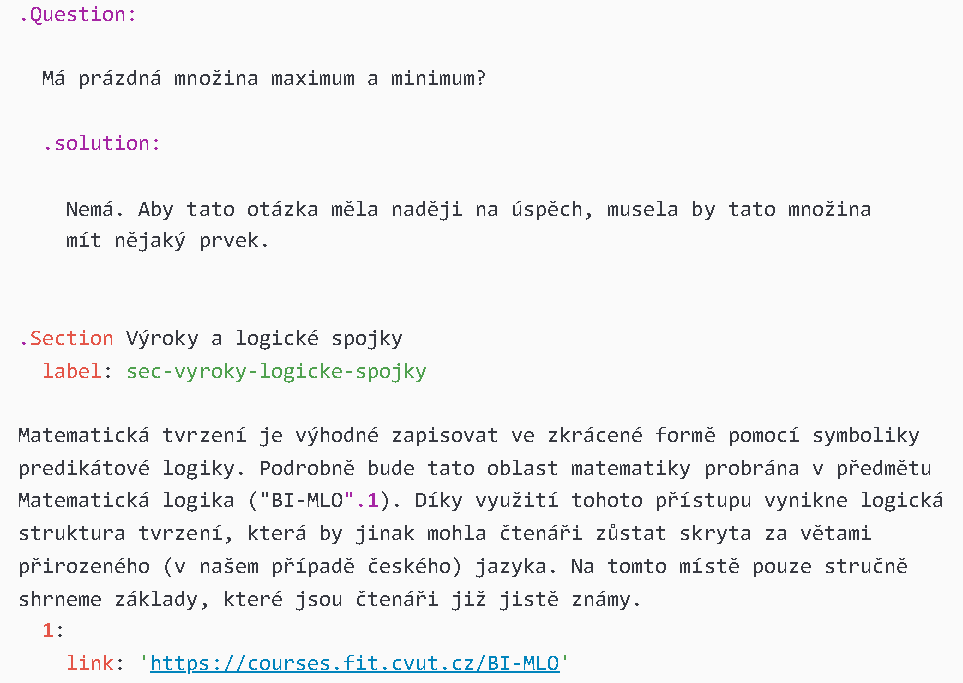
\includegraphics[width=1.0\textwidth]{content/realizace/zvýrazňování-syntaxe-pkm}
 	\caption[Zvýrazňování WooWoo syntaxe]{Zvýrazňování syntaxe WooWoo zdroje studijního textu k BI-PKM \cite{pkm}}
    \label{zvyraznovani-syntaxe-pkm}
\end{figure}

Podporována je také aktuální zkrácená forma vnitřních prostředí se zavináčem i starší zkrácená forma s tečkou. Jediným
prvkem WooWoo formátu, který není podporován, je direktiva \mintinline{text}{.include}.

Pro zajištění podpory napříč různými populárními tématy syntaxe byla použita pouze obvykle užívaná jména \textit
{scopes}, jejichž seznam uvádí \cite{textmate-grammars}.

\begin{sloppypar}
Vzhledem k omezeným vyjadřovacím schopnostem TextMate gramatik (které jsou založeny na rozšířených regulárních výrazech)
jsou některé konstrukty zvýrazňovány i tehdy, když nejsou zcela syntakticky správné. Například zvýrazňování syntaxe
verbózní formy vnitřních prostředí je řešeno zvýrazňováním ukončující části prostředí (horní dvojitá uvozovka
následovaná tečkou a typem prostředí). Na obrázku \ref{zvyraznovani-syntaxe-chyba-1} je ilustrován případ, kdy je
zvýrazněna syntaxe nevalidního vnitřního prostředí. Další chyby při zvýrazňování syntaxe jsou způsobeny nemožností
určit kontext. Jedna z takových chyb je ilustrována na obrázku \ref{zvyraznovani-syntaxe-chyba-2}, kde je chybně
zvýrazněno \uv{vnitřní prostředí} v křehkém vnějším prostředí.
\end{sloppypar}

\begin{figure}\centering
    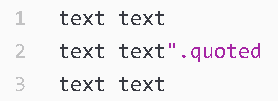
\includegraphics[width=0.35\textwidth]{content/realizace/zvýrazňování-syntaxe-chyba-1}
 	\caption[Chyba zvýrazňování syntaxe vnitřních prostředí]{Chyba zvýrazňování syntaxe WooWoo vnitřních prostředí}
    \label{zvyraznovani-syntaxe-chyba-1}
\end{figure}

\begin{figure}\centering
    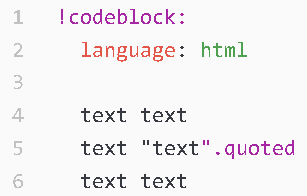
\includegraphics[width=0.35\textwidth]{content/realizace/zvýrazňování-syntaxe-chyba-2}
 	\caption[Chybějící kontext při zvýrazňování WooWoo syntaxe]{Chybějící kontext při zvýrazňování WooWoo syntaxe}
    \label{zvyraznovani-syntaxe-chyba-2}
\end{figure}
